\begin{problem}
Consider the function
\[
f(x,y) = xy.
\]
What is the shape of the level curve at height $0$ of $f$?
\begin{multipleChoice}
\choice{Empty}
\choice{A single line}
\choice[correct]{Two intersecting lines}
\choice{Two parallel lines}
\choice{Circle}
\choice{Ellipse}
\choice{Parabola}
\choice{Hyperbola}
\end{multipleChoice}

What is the shape of the level curve at height $1$ of $f$?
\begin{multipleChoice}
\choice{Empty}
\choice{A single line}
\choice{Two intersecting lines}
\choice{Two parallel lines}
\choice{Circle}
\choice{Ellipse}
\choice{Parabola}
\choice[correct]{Hyperbola}
\end{multipleChoice}

What is the shape of the level curve at height $-1$ of $f$?
\begin{multipleChoice}
\choice{Empty}
\choice{A single line}
\choice{Two intersecting lines}
\choice{Two parallel lines}
\choice{Circle}
\choice{Ellipse}
\choice{Parabola}
\choice[correct]{Hyperbola}
\end{multipleChoice}

What is the shape of the level curve at height $2$ of $f$?
\begin{multipleChoice}
\choice{Empty}
\choice{A single line}
\choice{Two intersecting lines}
\choice{Two parallel lines}
\choice{Circle}
\choice{Ellipse}
\choice{Parabola}
\choice[correct]{Hyperbola}
\end{multipleChoice}

Which of the following is the graph of $f$?

\begin{image}
\begin{tikzpicture}
\node[inner sep=0pt] at (0,0)
    {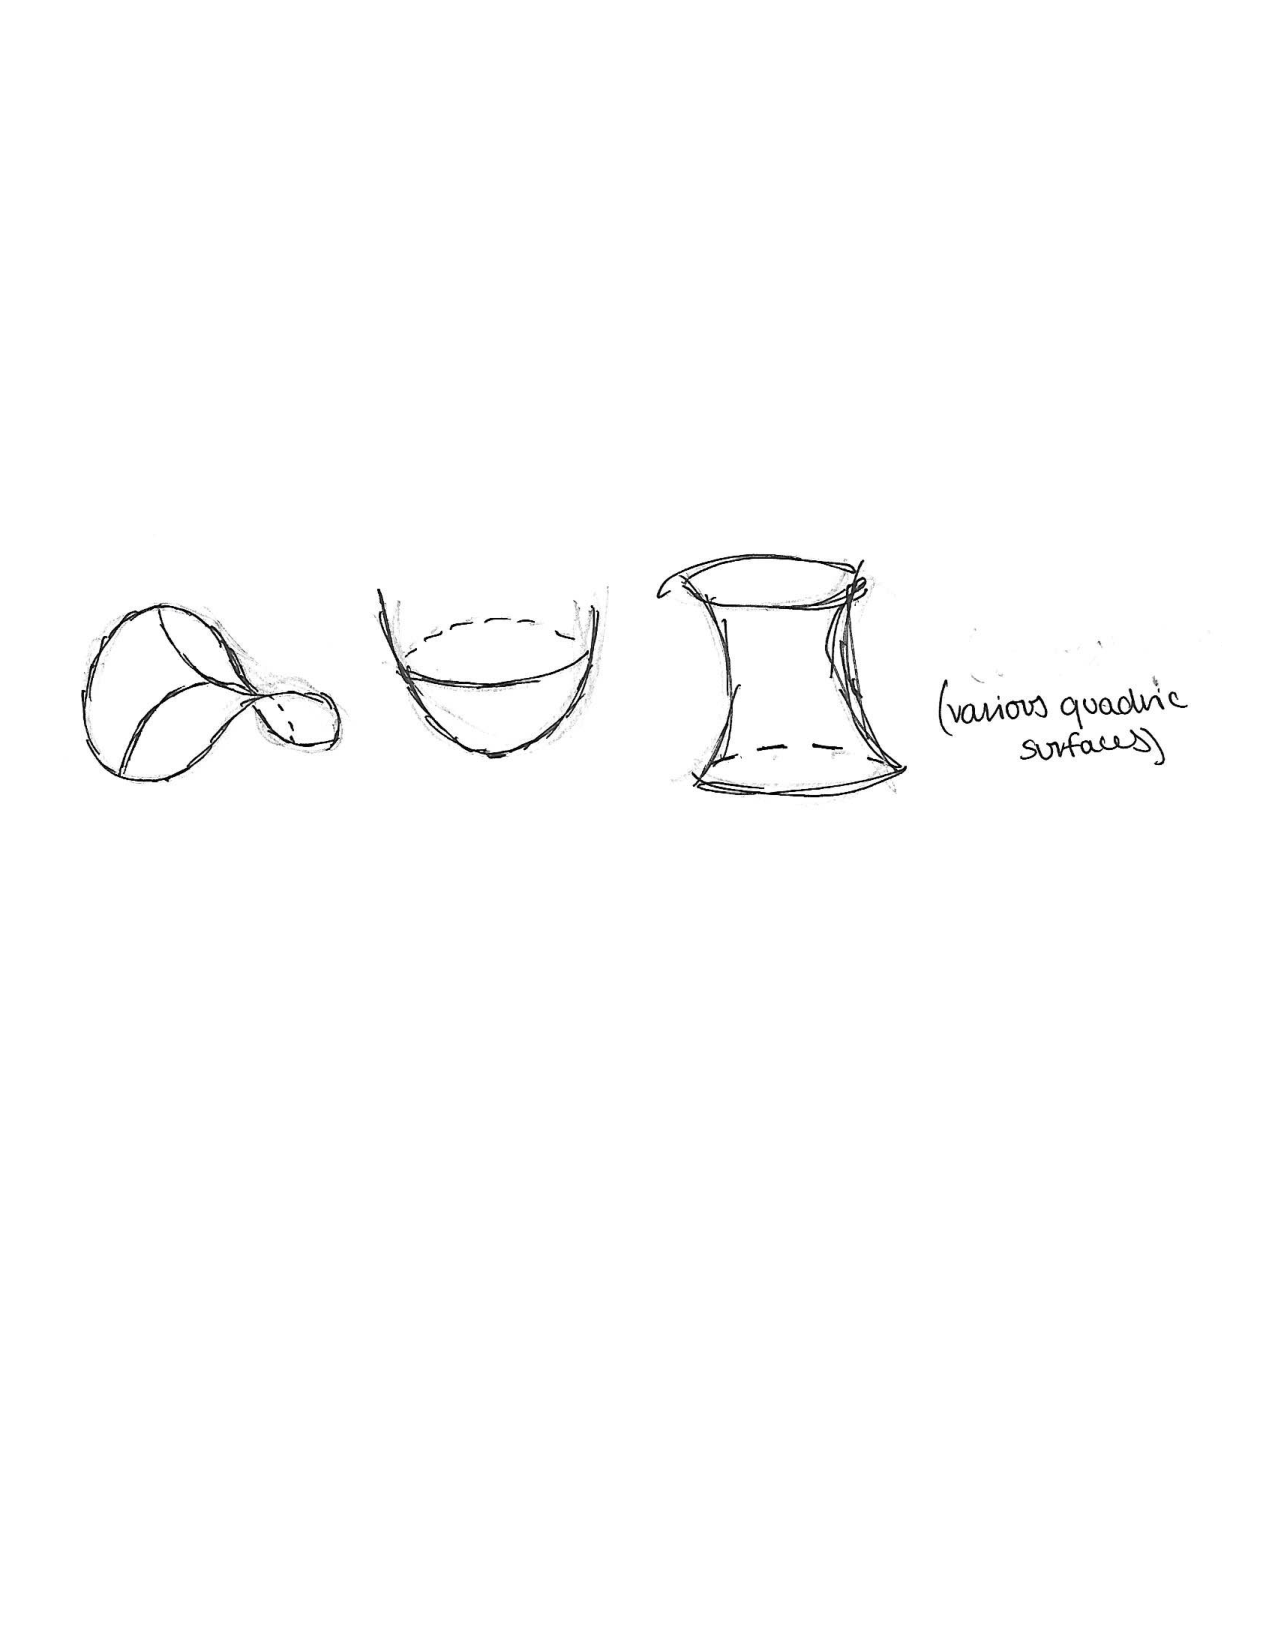
\includegraphics{quadric_options}};
\end{tikzpicture}
\end{image}
\end{problem}